The syntax has been designed to use as less XML elements as possible and to rely on XML attributes to setup the element behavior in a particular context.
As shown in \ref{tbl:syntax-ele} the mapping elements  can be grouped in 3 different scopes. There are only 3 elements for the models structure itself. We assume that any data hierarchy  can be represented a combination of collections (COLLECTION), tuples (INSTANCE) and simple values (ATTRIBUTE). The others elements are either set the mapping block structure or to connect data to each other.

\begin{table}[!htbp]
\small
\centering
\begin{tabulary}{\linewidth}{|c|J|}       
       \hline 
            \textbf{Scope} & 
            \textbf {Elements}\\
       \hline         
       \hline  
             Data modeling tags & 
             ATTRIBUTE INSTANCE COLLECTION \\
       \hline  
             Mapping block structre & 
             VODML MODEL REPORT TEMPLATES GLOBALS \\
       \hline  
             Data references and identification & 
             REFERENCE JOIN  FOREIGN\_KEY PRIMARY\_KEY WHERE\\
       \hline
     \end{tabulary}
     \caption{Mapping elements grouped by scopes} 
     \label{tbl:syntax-ele}
\end{table}


As shown in \ref{tbl:syntax-att} and following the VODML pattern, any model node is characterized by a role (@dmrole) and a type (@dmtype). All of the others attributes are used to bind data with either VOtable elements or others mapping elements.
 
\begin{table}[!htbp]
\small
\centering
\begin{tabulary}{\linewidth}{|c|J|}       
       \hline 
            \textbf{Scope} & 
            \textbf {Attributes}\\
       \hline         
       \hline  
             Model related & 
             @name @uri \\
       \hline  
             Modeled node related & 
             @dmrole @dmtype \\
       \hline  
             Related to attribute values & 
             @value @unit @arrayindex \\
       \hline  
             Related to VOTable elements & 
             @tableref @ref\\
       \hline  
             Mapping element identification& 
             @dmref @dmid @url @dmid @sourceref @primarykey @foreignkey\\
       \hline
     \end{tabulary}
     \caption{Attributes of mapping elements grouped by scopes} 
     \label{tbl:syntax-att}
 \end{table}
 
 


  \begin{figure}[h]
    \begin{center}
      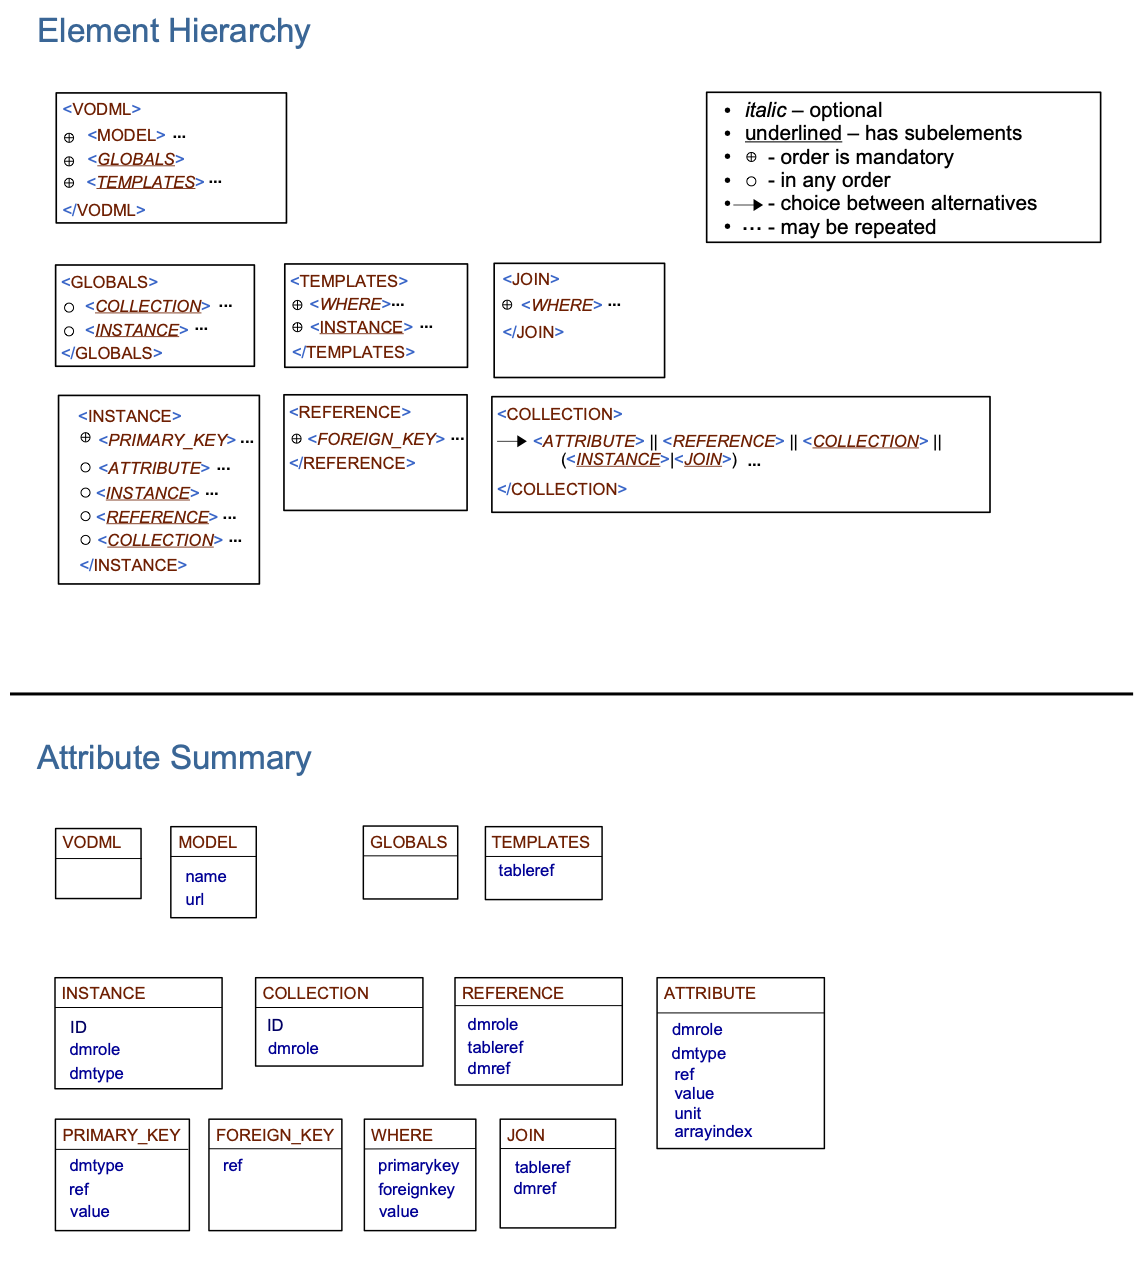
\includegraphics[width=\textwidth]{merged-syntax-summary.png}
      \caption{Annotation Syntax Summary}
      \label{fig:summary}
    \end{center}
  \end{figure}
